\section{Exercício 2 -- Introdução ao Pytorch Convnet}

\begin{itemize}
	\item Notebook: \textit{introducing-pytorch-convnet.ipynb}
\end{itemize}

\subsection{Descrição}

O notebook em questão contém uma série de demonstrações de conceitos básicos do Pytorch, como as operações de convolução, a função de ativação, \textit{pooling}. Além de \textit{skip connections}, camadas densamente conectadas, \textit{dropout} etc. Por fim, há um processo de construção e treinamento de uma rede neural, desde sua construção, definição de função de perda e otimizador, processo de treinamento e validação.

O problema do processo que foi realizado é que houve \textit{overfitting} (Figura~\ref{fig:note2:init_train}), noticiado pelo custo de treinamento consistentemente menor do que o de validação. O exercício em questão consiste numa exploração dos elementos e hiperparâmetros utilizados para melhorar o resultado obtido. A acurácia inicial é de 0,93.

\begin{figure}[!htb]
	\centering
	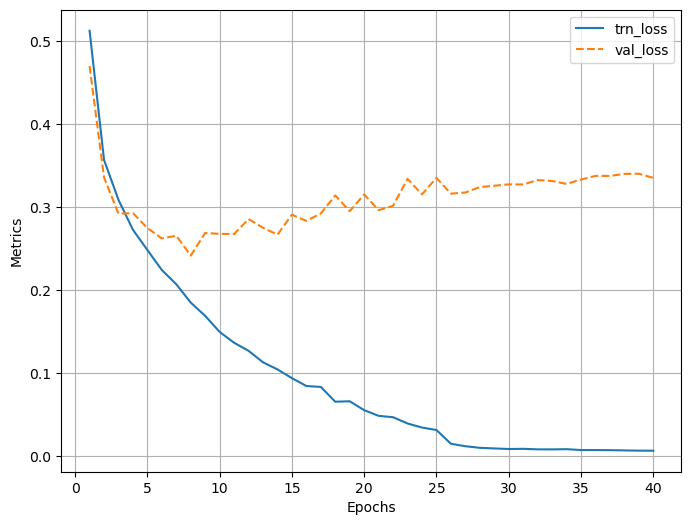
\includegraphics[width=0.6\linewidth]{intro_convnet/initial_train}
	\caption{Gráfico do custo de treinamento e de validação ao longo das épocas de treinamento.}
	\label{fig:note2:init_train}
\end{figure}

\subsection{Resolução do Exercício Proposto}

Como está ocorrendo um fenômeno de \textit{overfitting}, a primeira alteração feita foi aumentar a regularização L2 o otimizador, alterando o valor de \textit{weight\_decay} para $0,001$ (antes era $0,0001$). Contudo o efeito não foi positivo, a acurácia foi de 0,928 e o \textit{overfitting} permaneceu (Figura~\ref{fig:intro_conv:train}-a), portanto a alteração foi descartada.

Em seguida, a probabilidade da operação de \textit{dropout} foi aumentada, de 20\% para 50\% de chance de desconectar uma ligação da camada densa. A acurácia não apresentou melhoria, permaneceu em 0,93, mas o efeito de \textit{overfitting} pareceu ser atenuado (Figura~\ref{fig:intro_conv:train}-b), mesmo que ainda não solucionado. De qualquer forma, a alteração foi mantida.

Por fim, a última modificação testada foi adicionar algumas operações de \textit{data augmentation} no conjunto de treinamento. Para isso, foi feito uma classe de \textit{dataset} personalizada, que funciona como \textit{wrapper} da original, mas podendo aplicar \textit{data augmentation} apenas no conjunto de treinamento.

Foram adicionadas duas operações: (i) com uma chance de 50\%, pode ocorrer uma flip horizontal da imagem; (ii) é aplicado um filtro gaussiano com tamanho de kernel 3 e sigma aleatório entre 0,1 e 2. Com essa abordagem, os efeitos do sobreajuste foram bastante minimizados (Figura~\ref{fig:intro_conv:train}-c), mas a eficácia obtida permaneceu perto em 93\%, sugerindo um possível limite para esse modelo.

Remover da arquitetura a \textit{skip connection} não teve efeito e remover uma das camadas convolucionais piorou levemente o resultado. Talvez a melhor coisa a ser feita seja trocar por completo a rede neural utilizada.



\begin{figure}[!htb]
	\centering
	\subfloat[\textit{$\text{weight\_decay} = 0,001$}]{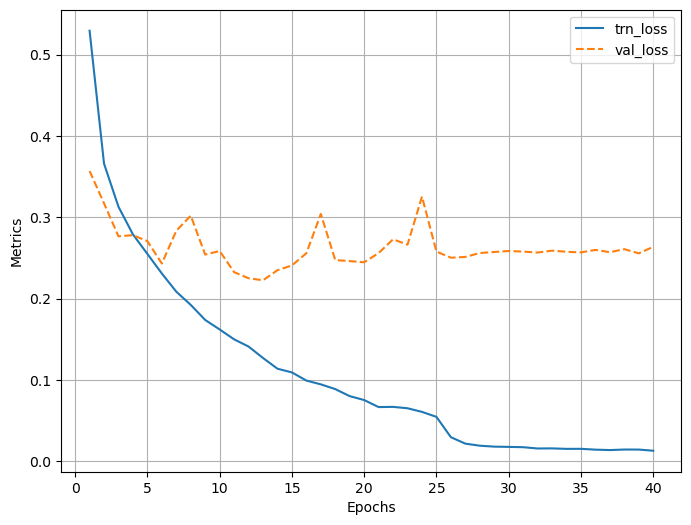
\includegraphics[width=0.45\linewidth]{intro_convnet/increase_l2}}
	\subfloat[$\text{dropout} = 0,5$]{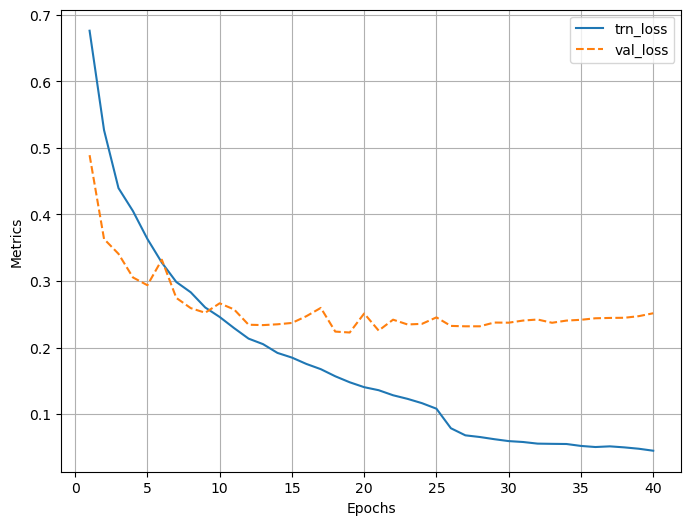
\includegraphics[width=0.45\linewidth]{intro_convnet/drop_0_5}} \\
	\subfloat[\textit{Data Augmentation}]{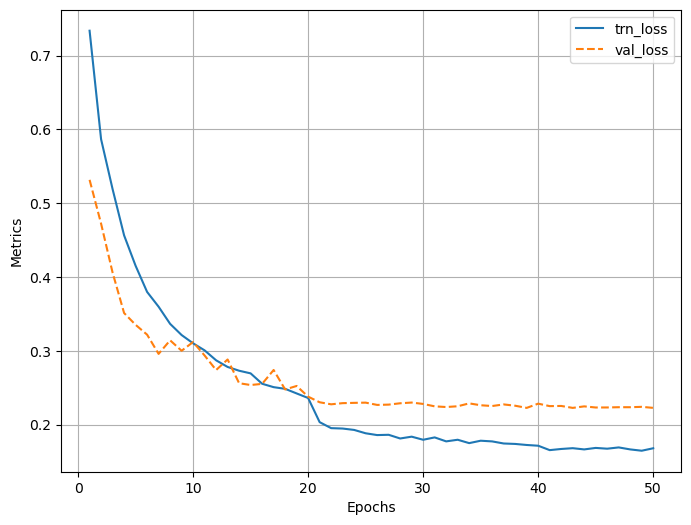
\includegraphics[width=0.45\linewidth]{intro_convnet/aug}}
	\caption{Gráfico do custo de treinamento e de validação ao longo das épocas de treinamento para diferentes modificações no modelo.}
	\label{fig:intro_conv:train}
\end{figure}